\documentclass{scrartcl}

\usepackage{graphicx}

\usepackage[backend=biber, style=numeric-comp]{biblatex}
\addbibresource{references.bib}

\usepackage{authblk}

\parindent0em
\parskip1em

\usepackage{enumitem}
\setlist{nosep}

\begin{document}

\title{Results of the un-deRSE 2023 Breakout Session “RSE Educational Resource Discoverability”}
\author[1]{Toby Hodges}
\affil[1]{The Carpentries}

\author[2]{Christian Knüpfer}
\affil[2]{Friedrich Schiller University Jena}

\author[3]{Michele Mesiti}
\affil[3]{Karlsruhe Institute of Technology}

\author[4]{David Pape}
\affil[4]{Helmholtz-Zentrum Dresden-Rossendorf}

\author[2]{Philipp Matthias Schäfer}

\author[5]{Tobias Schlauch}
\affil[5]{German Aerospace Center}

\author[6]{Philipp S. Sommer \footnote{This list of authors includes those persons that were present at the workshop and indicated their wish to be listed. There were others who contributed as well.}}
\affil[6]{Helmholtz-Zentrum Hereon}


\date{28. September 2023}
\maketitle

During the breakout session, we, the participants, discussed three questions and answered them in the form of collections of notes organized on pin boards.

After a short introduction of the issue under discussion, we split the group in two halves and discussed the questions
\begin{itemize}
\item What standards, tools, and infrastructure exists?
\end{itemize}
and
\begin{itemize}
\item What information are we interested in when looking for resources?
\end{itemize}
(both in the context of research software engineering (RSE) educational resources (ER) discoverability).
Each half worked on both questions, then we rejoined and summarized the results.

Finally, building on our these results, we discussed the third question:
\begin{itemize}
\item What is missing and how could we go about creating it?
\end{itemize}

The rest of this document consists of one section per question discussed, presenting our results, which are mostly collections of keywords and references, occasionally with comments.

\section*{What standards, tools, and infrastructure exists?}

Answers to this question were not restricted to existing standards, tools, and infrastructure that are directly applicable to RSE ER, but rather anything that we might build upon or draw inspiration from was allowed.
Figure~\ref{fig:existing} shows a cropped photograph of the pin board for this question at the end of the session.

\begin{figure}[h]
  \centering
  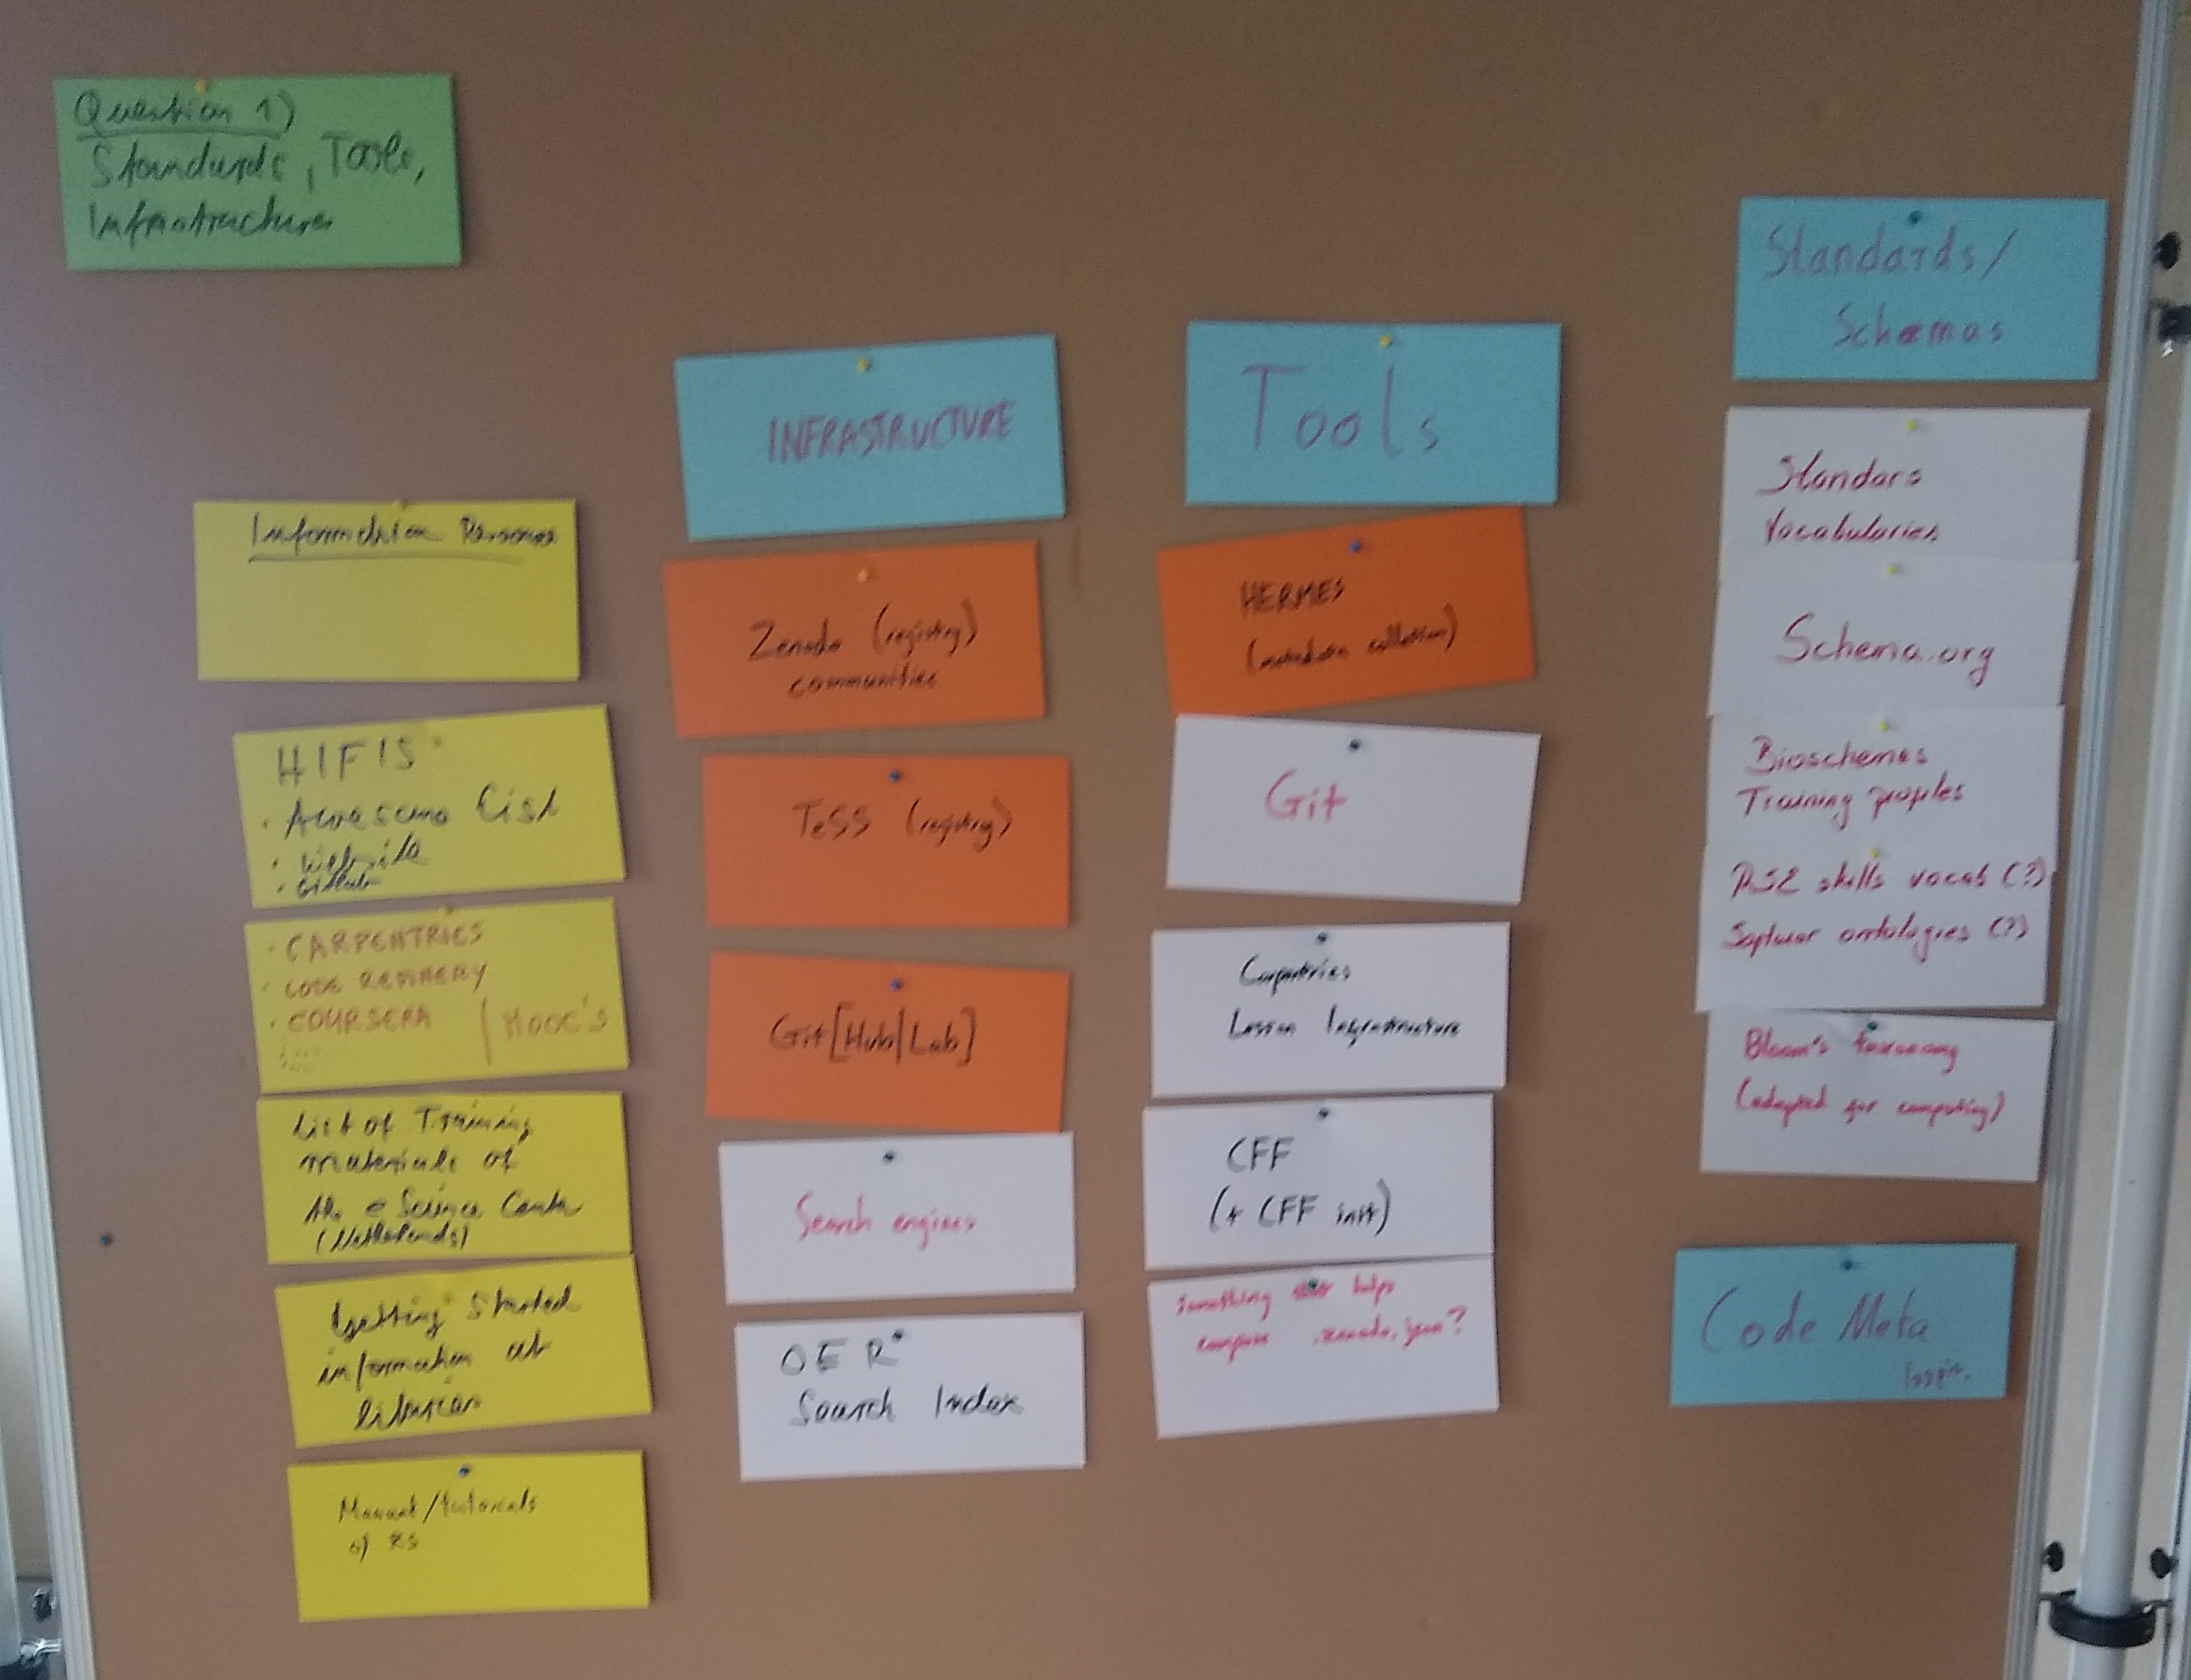
\includegraphics[width=0.9\textwidth]{existing}
  \caption{Pin Board with our answers to “What standards, tools, and infrastructure exists?”}\label{fig:existing}
\end{figure}

In addition to standards, tools, and infrastructure, we added a category, information resources, under which we collected current documents that list and link to or host existing ER:
\begin{itemize}
\item HIFIS \cite{HifisMaterial}
\item The Carpentries \cite{CCLessons, DCLessons, LCLessons, SWCLessons}
\item CodeRefinery \cite{CRLessons}
\item Many MOOC-platforms offer courses on topics relevant to RSE
\item eScienceCenter - Training materials \cite{eSSMaterial}
\item getting started information of libraries
\item Manuals/Tutorials of RStudio \cite{RSGuides}
\end{itemize}

We collected the following notes on existing standards:
\begin{itemize}
\item Standard Vocabularies
\item Schema.org
\item Bioschemas’ Training profiles \cite{castro2023bioschemas}
\item RSE skill vocabularies
\item Software ontologies
\item Bloom’s taxonomy adapted for computing
\item CodeMeta \cite{CMProject}
\end{itemize}

We collected the following notes on existing tools:
\begin{itemize}
\item Hermes \cite{Meinel_hermes}, which is already being adapted to generate metadata for educational resources
\item Git, as a provider of metadata on contributors
\item Carpentries Lesson Infrastructure \cite{CWB}, which does/will generate and incorporate metadata using Hermes in the compiled educational resources
\item CFF \cite{druskat2021citation, CFF} with CFF init \cite{Spaaks_cffinit_2023} as inspiration
\end{itemize}

We collected the following notes on existing infrastructure:
\begin{itemize}
\item Zenodo communities
\item TeSS \cite{beard2020tess, TESS}
\item Git[Hub|Lab]
\item Search engines
\item OERSI.org \cite{OERSI}, an existing registry
\end{itemize}

\section*{What information are we interested in when looking for resources?}

Figure~\ref{fig:metadata} shows a cropped photograph of the pin board for this question at the end of the session.

\begin{figure}[h]
  \centering
  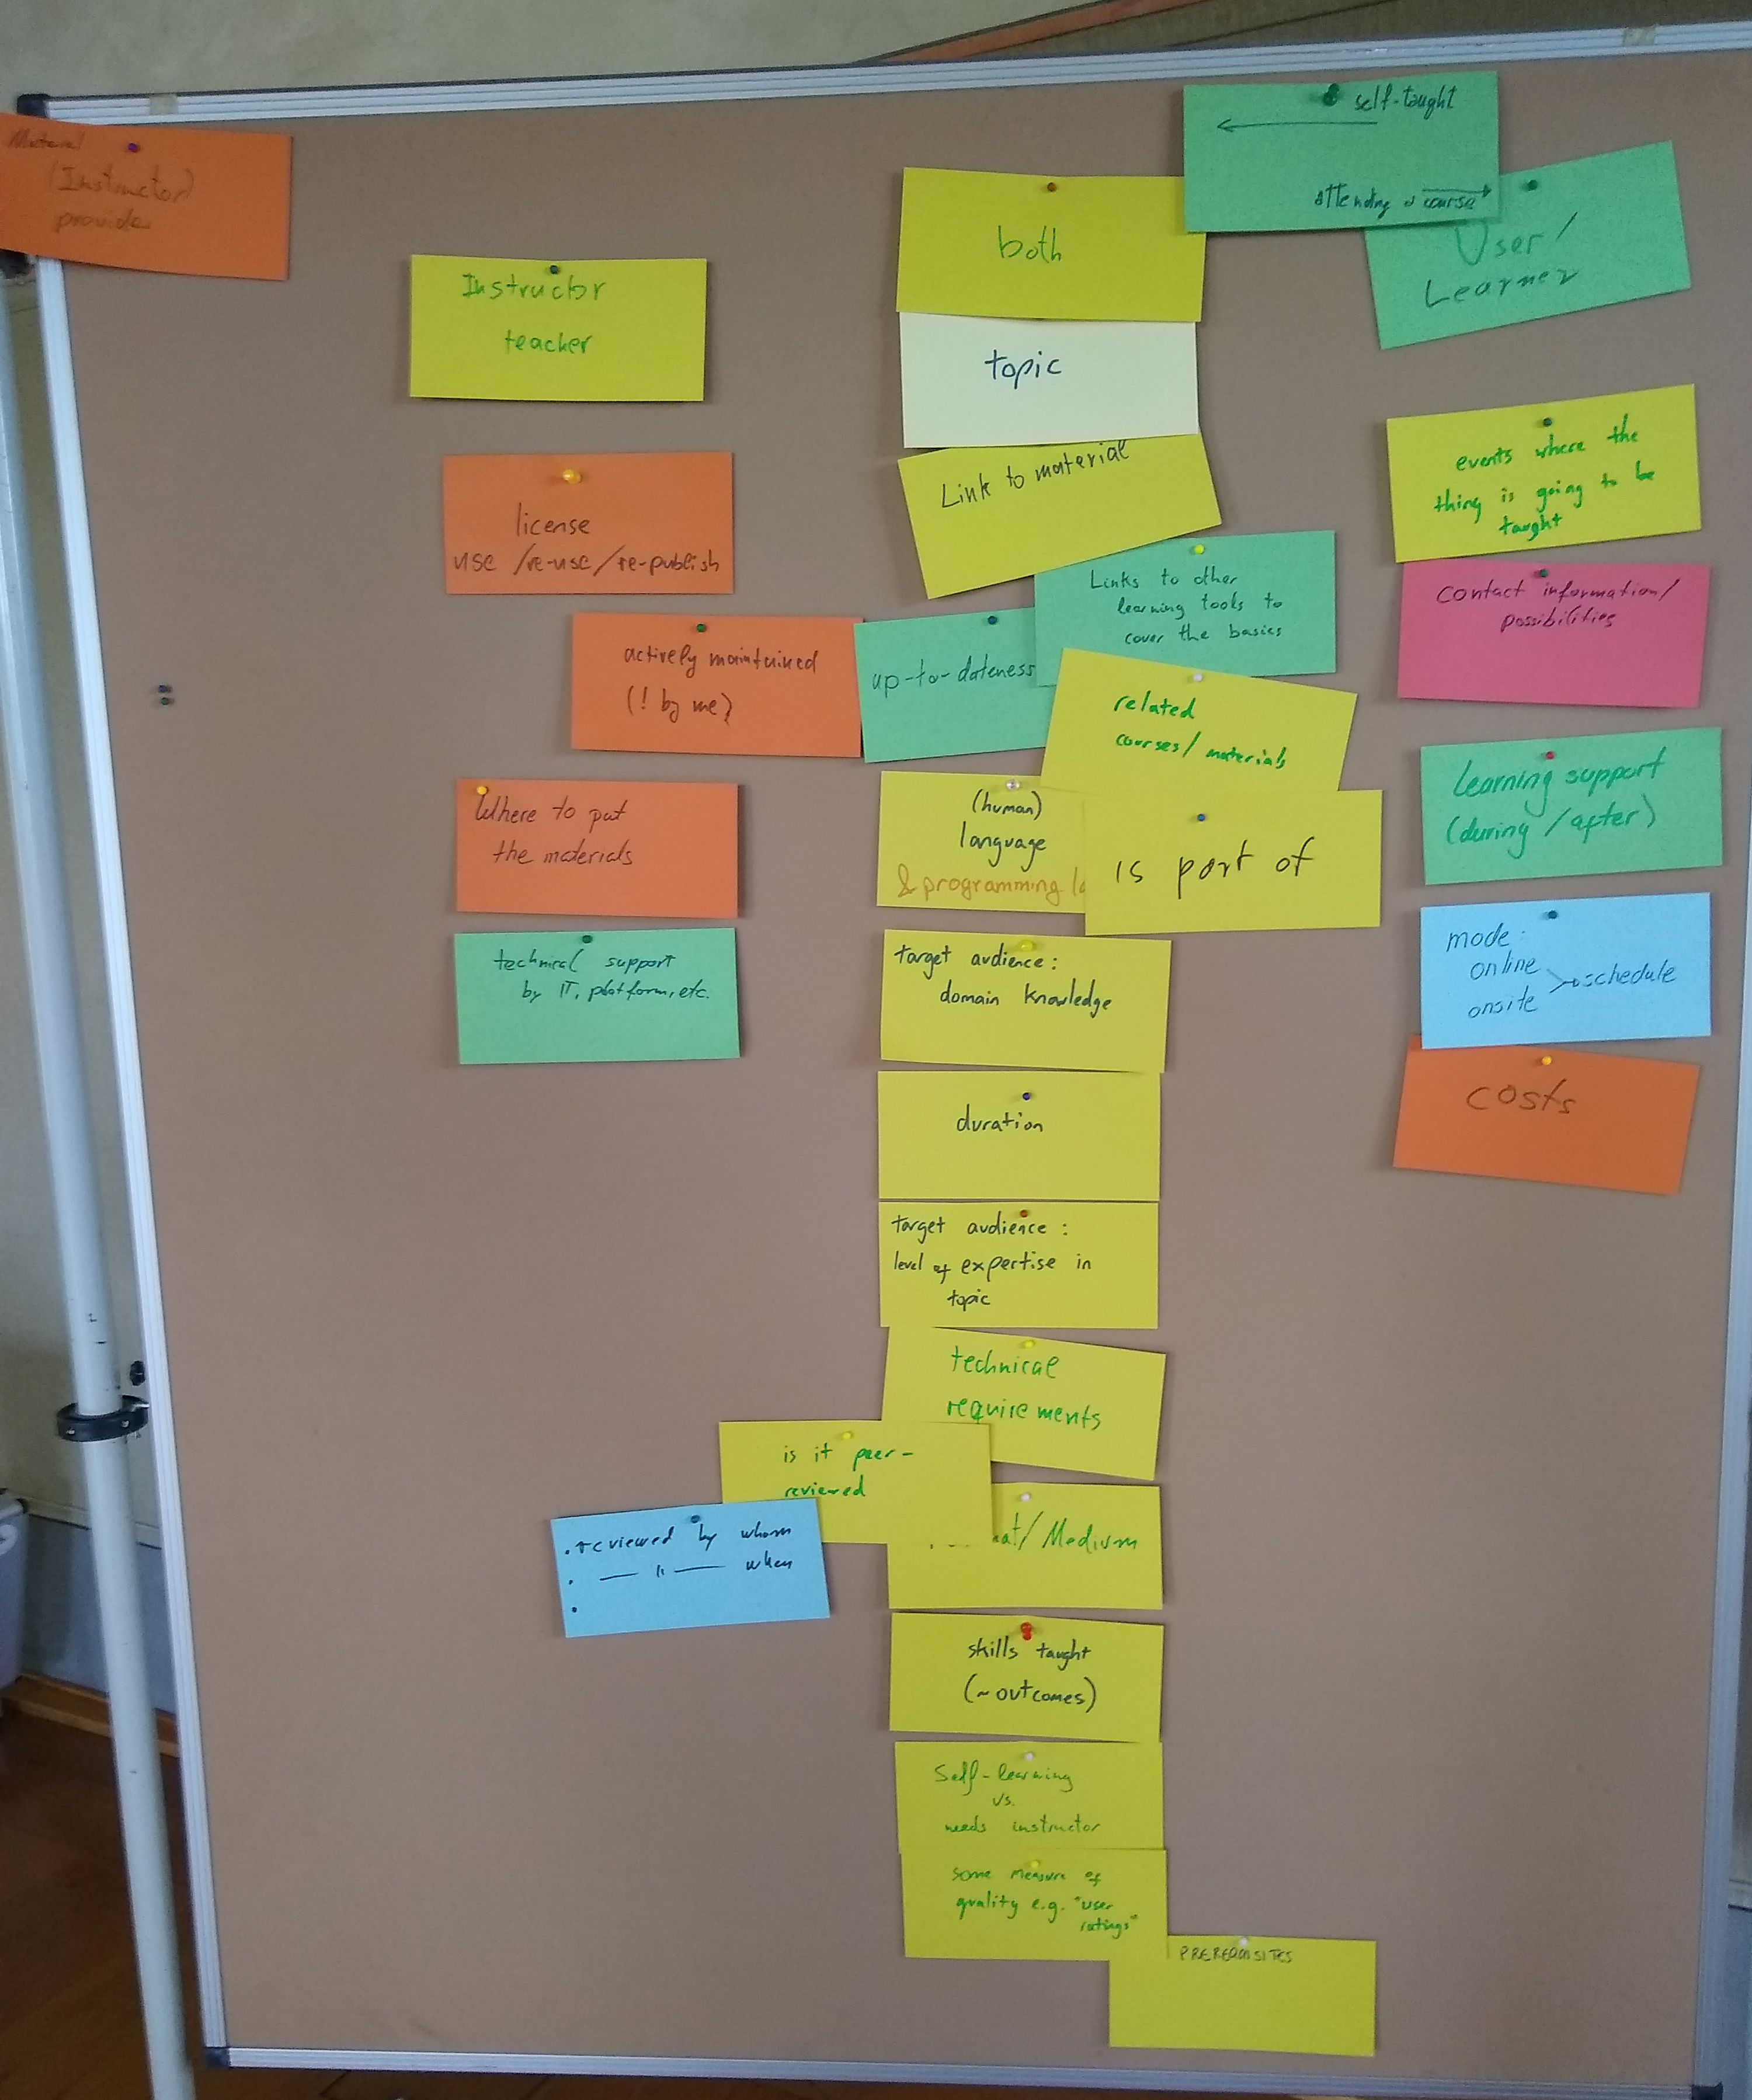
\includegraphics[width=0.9\textwidth]{metadata}
  \caption{Pin Board with our answers to “What information are we interested in when looking for resources?”}\label{fig:metadata}
\end{figure}

We collected desired information in three categories: that which teachers are interested in when searching, that which learners are interested in, and that which both are interested in.
We briefly thought about a fourth category covering providers (authors and maintainers) of material, but as they are usually not searching for that material in these roles, they should be interested in providing metadata that satisfies the other groups interests.

For both roles, teacher and learner, we expect the following information to be of interest:
\begin{itemize}
\item topic
\item link to the resource itself
\item up-to-dateness
\item references/links to related resources (prerequisites/follow-ups)
\item language
\item duration
\item is-part-of relationship (episode of a course, for example)
\item target audience: required level of expertise
\item target audience: domain
\item technical requirements
\item peer review information (who/when)
\item format/medium (video, course notes, slides, etc.)
\item outcomes: skills taught
\item suitability for self-learning/teaching
\item measure of quality/user rating
\end{itemize}

Only for teachers, we expect the following information to be of interest:
\begin{itemize}
\item license regarding use, reuse, and republishing the resource
\item active maintenance
\item references to technical support by IT, the platform, etc.
\end{itemize}

The information that we think only learners are interested in, mostly revolves around courses that use the resource:
\begin{itemize}
\item events, that teach based on the resources
\item contact information
\item references to learner support during and after courses
\item mode of courses (online, onsite, hybrid)
\item cost of courses
\item schedule of courses
\end{itemize}

\section*{What is missing and how could we go about creating it?}

Figure~\ref{fig:future} shows a cropped photograph of the pin board for this question at the end of the session.

\begin{figure}[h]
  \centering
  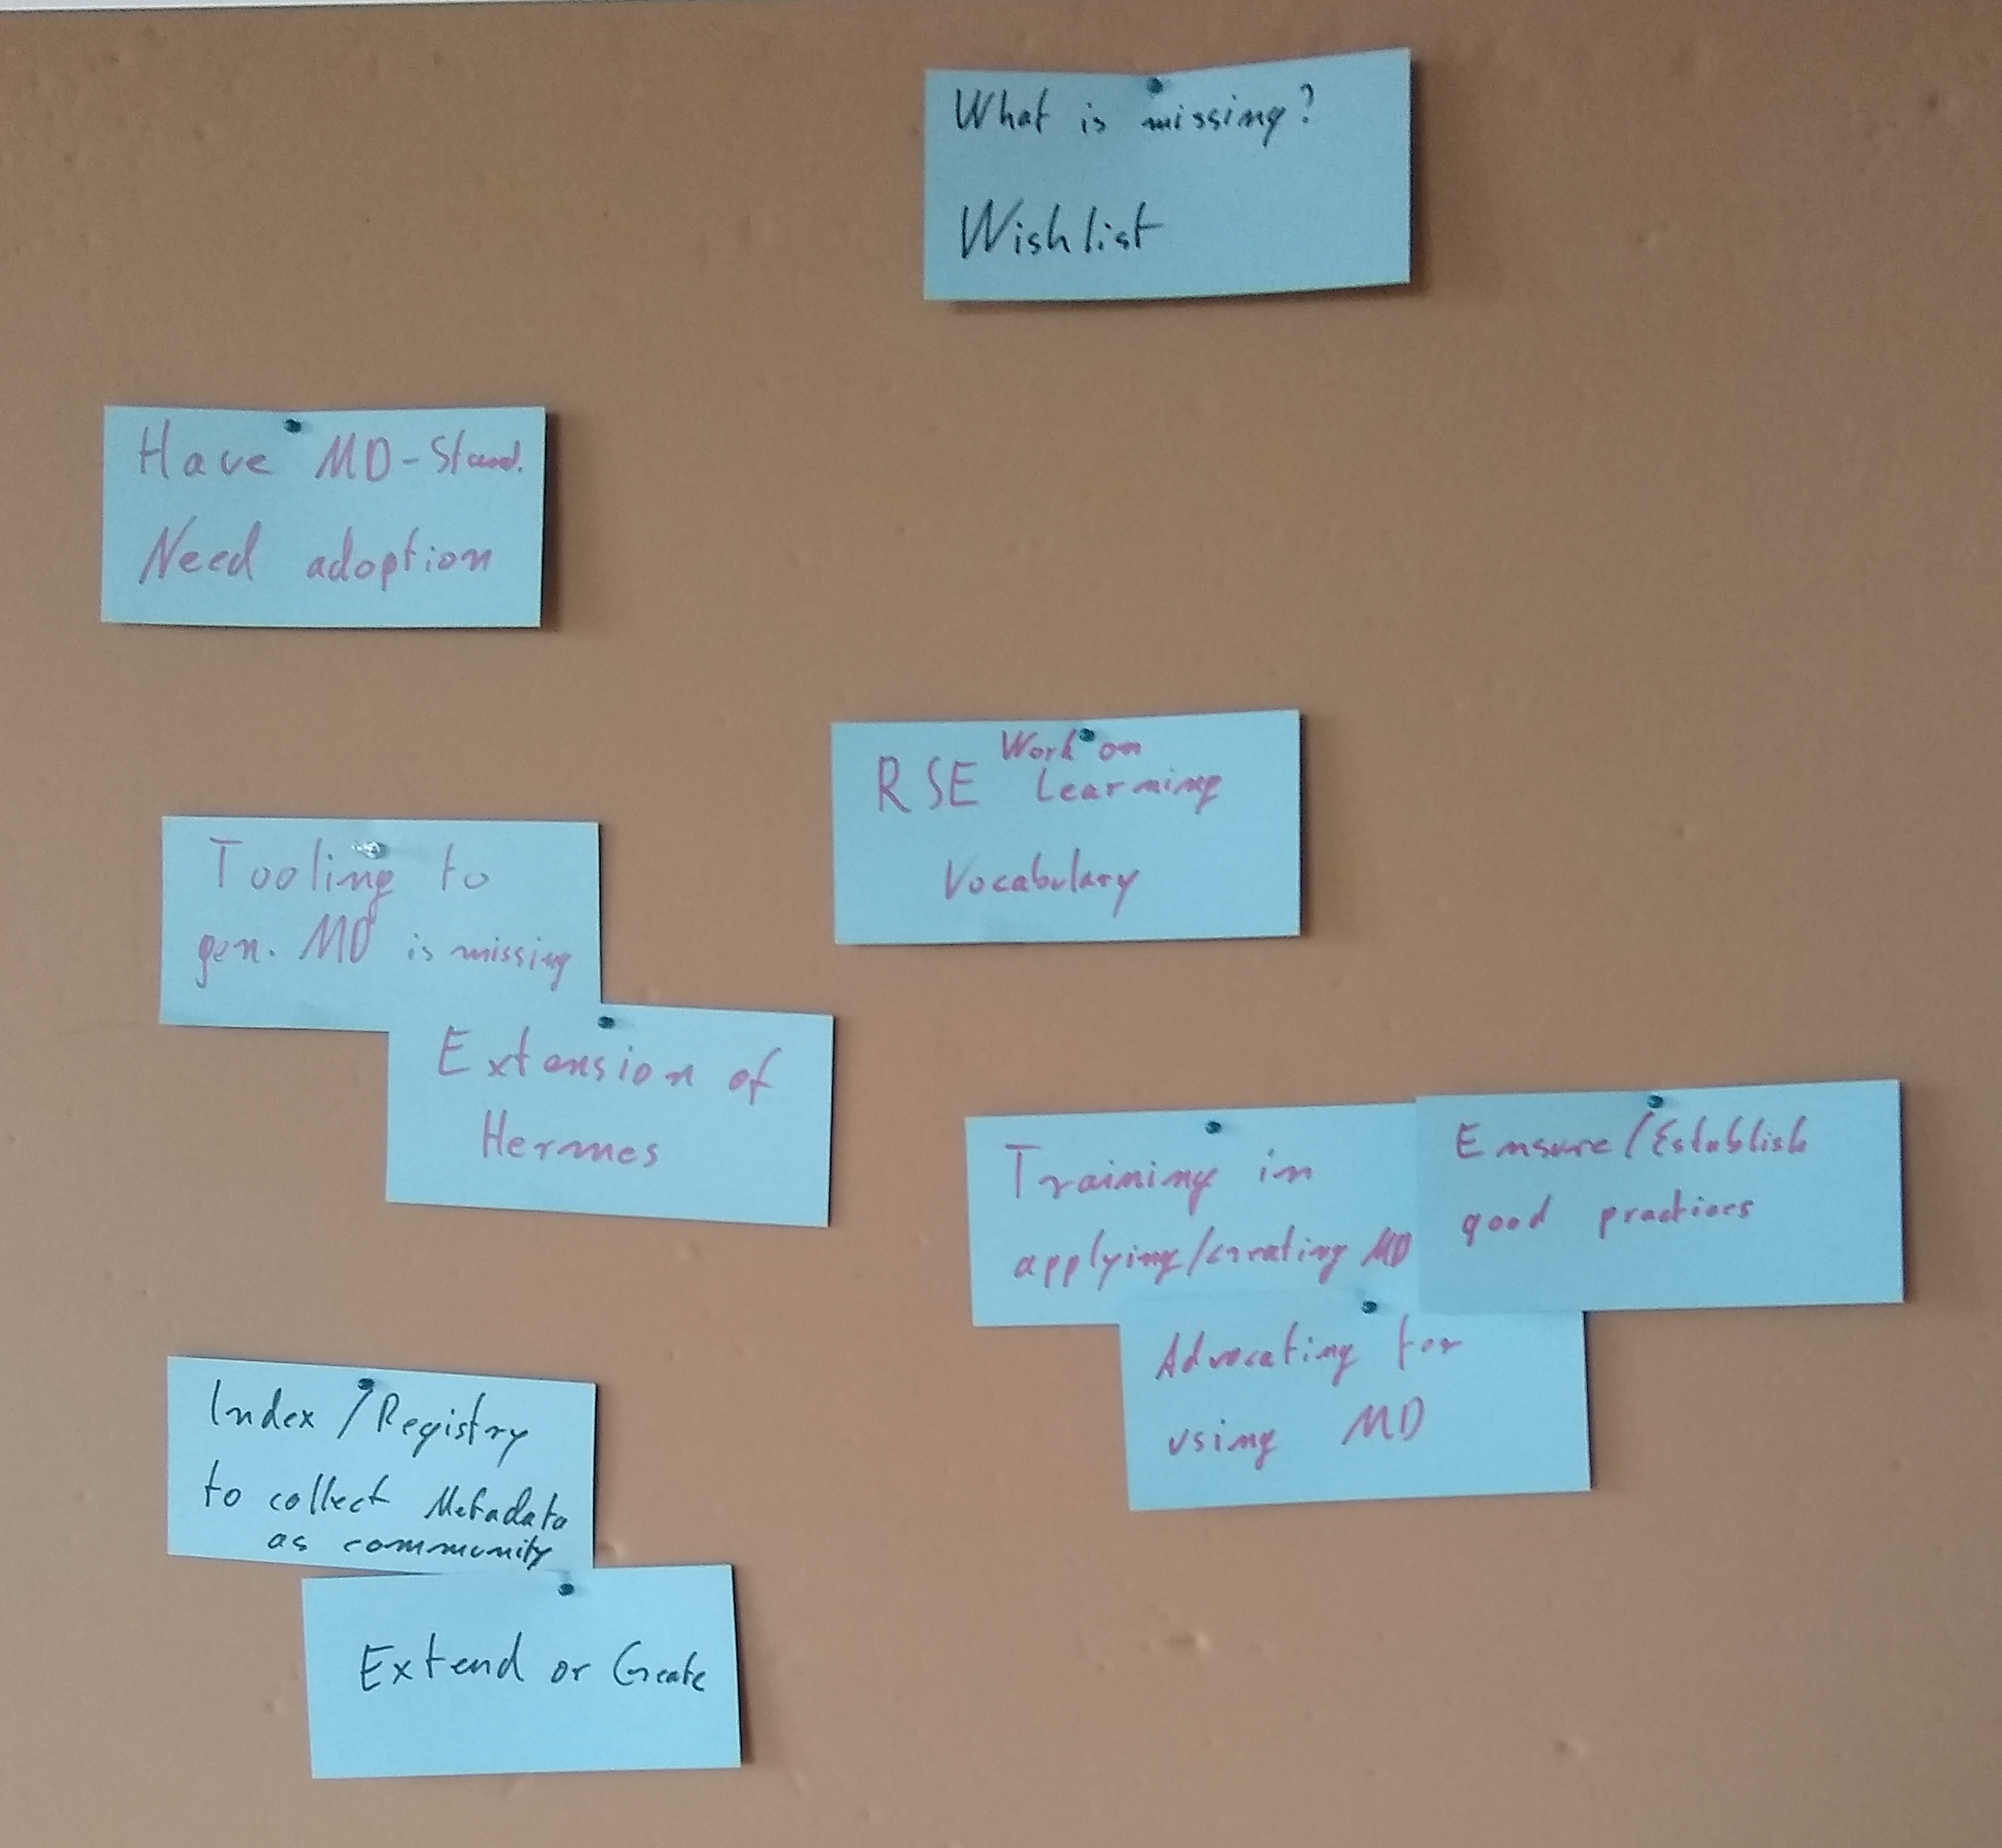
\includegraphics[width=0.9\textwidth]{future}
  \caption{Pin Board with our answers to “What is missing and how could we go about creating it?”}\label{fig:future}
\end{figure}

For next steps or their desired outcomes we collected the following list:
\begin{itemize}
\item work on RSE learning vocabulary
\item metadata standard for RSE ER with adoption in the community
\item training for applying and creating metadata to ensure and establish good practices
\item advocating use of metadata standard
\item tooling to generate metadata for RSE ER (an extension of Hermes\cite{Meinel_hermes} has already been worked on)
\item extend or create an index or a registry in which the RSE community collects metadata on ER
\end{itemize}

\printbibliography

\end{document}

%%% Local Variables:
%%% coding: utf-8
%%% mode: latex
%%% TeX-engine: xetex
%%% End:
